\documentclass[letter]{llncs}
\usepackage{capt-of}

\newcommand{\figshrink}{\vspace{-.6cm}}
%\newcommand{\figshrinkend}{\vspace{-.4cm}}
\newcommand{\figshrinkend}{}
\usepackage{amssymb}
\usepackage{times}
\setcounter{tocdepth}{3}
\usepackage{graphicx}
\usepackage{amsmath}
\usepackage{listings}
\usepackage{enumerate}
\usepackage{textcomp}
\usepackage[caption=false,font=footnotesize]{subfig}
\usepackage{lipsum}

\usepackage{algpseudocode}% http://ctan.org/pkg/algorithmicx
\usepackage{algorithm}
\usepackage{amsmath}
\usepackage{url}

\newcommand{\Tr}{\ensuremath{\mathsf{TrS}}}
\newcommand{\TrR}{\ensuremath{\mathsf{TrR}}}
\newcommand{\TrA}{\ensuremath{\mathsf{Cond}}}
\renewcommand{\a}[1]{\ensuremath{\mathsf{#1}}}
\newcommand{\concat}{\ensuremath{\mathop{+\!\!+}}}
%\newcommand{\figshrinkend}{\vspace{-.4cm}}
\newcommand{\secshrink}{\vspace{-.5cm}}
\newcommand{\secshrinkbegin}{\vspace{-.2cm}}
\newcommand{\subsecshrink}{\vspace{-.5cm}}
\newcommand{\subsecshrinkbegin}{\vspace{-.2cm}}
\setlength{\abovecaptionskip}{1ex}
\setlength{\belowcaptionskip}{1ex}
\setlength{\floatsep}{1ex}
\setlength{\textfloatsep}{1ex}

\setcounter{tocdepth}{3}

\makeatletter
\renewcommand{\ALG@beginalgorithmic}{\small}
\algrenewcommand\algorithmicindent{0.5em}%
\makeatother

\DeclareMathSizes{10}{10}{9}{9}

\begin{document}

\title{Property Specification Made Easy: Harnessing the Power of Model Checking in UML designs}

  \author{Daniela Remenska\inst{1,3}
  \and Tim A.C. Willemse\inst{2} \and \\ Jeff Templon\inst{3} \and\
  Kees Verstoep\inst{1} \and Henri Bal\inst{1}}
%
% (feature abused for this document to repeat the title also on left hand pages)

% the affiliations are given next; don't give your e-mail address
% unless you accept that it will be published
\institute{Dept. of Computer Science, VU University Amsterdam, The Netherlands
\and
Dept. of Computer Science, TU Eindhoven, The Netherlands
\and
NIKHEF, Amsterdam, The Netherlands
}

\maketitle

\begin{abstract}
Developing correct concurrent software is challenging. Design errors
can result in deadlocks, race conditions and livelocks, and discovering
these is difficult.  A serious obstacle for an industrial uptake of rigorous analysis
techniques such as model checking is the steep learning curve associated
to the languages --- typically temporal logics --- used for specifying the
application-specific properties to be checked. To bring the process of
correctly eliciting functional properties closer to software engineers,
we introduce PASS, a Property ASSistant wizard as part of a UML-based
front-end to the mCRL2 toolset. PASS instantiates pattern templates using
three notations: a natural language summary, a $\mu$-calculus formula
and a UML sequence diagram depicting the desired behavior. Most approaches to date 
have focused on LTL, which is a state-based formalism. Conversely,
 $\mu$-calculus is event-based, making it a good match for sequence diagrams, where communication between
 components is depicted. We revisit a case
study from the Grid domain, using PASS to obtain the formula and monitor
for checking the property.
%%
%%Early discovery of design errors which can lead to deadlocks or race conditions is 
%%challenging in concurrent software development. 
%%In the last decades, more rigorous
%%methods and tools for modeling and formal analysis have been developed. 
%%Although approaches for automatically generating formal models from system designs have 
%%been proposed, another serious obstacle for adopting model checking tools in industry
%%is the formulation of application-specific properties to be checked. 
%%This requires expertise in temporal logic, regardless of the verification tool used.
%%To bring the process of correctly eliciting functional properties closer to software 
%%designers, we introduce PASS, a Property ASSistant wizard developed 
%%as an Eclipse plugin. Our starting point was the well-established property pattern system,
%%which we extended with new property templates, to capture variations not covered 
%%in the original classification. PASS instantiates pattern templates using three notations: a natural language summary, a $\mu$-calculus formula
%%and a UML sequence diagram depicting the desired behavior. Most approaches to date 
%%have focused on LTL, which is a state-based formalism. Conversely,
%% $\mu$-calculus is event-based, making it a good match for sequence diagrams, where communication between
%% components is depicted. 
%%Moreover, such communication is data-dependent, so we introduce
%%the possibility to define data quantifiers, to express complex properties in a concise manner.
%%To cope with state-space explosion, we provide one additional notation: a monitor for on-the-fly model checking, or bug hunting.
%%We revisit a case study from the Grid domain, using PASS to obtain the
%%formula and monitor for checking the property with mCRL2.
% \keywords{property specification, model checking, UML, sequence diagrams, modal
% $\mu$-calculus, property patterns}
\end{abstract}
\vspace{-20 pt}

\section{Introduction}
\vspace{-10 pt}

\label{sec:Introduction}
A challenge during the development of concurrent systems is detecting
design errors, as such errors can cause deadlocks, livelocks, race conditions,
starvation, etc. The sheer number of different executions and the
inherent non-determinism in concurrent systems make complete testing of such software
infeasible. Instead, more rigorous formal analysis techniques like
model checking are required, which exhaustively analyze the behaviors of 
(an abstraction of) the system. Toolsets such as SPIN, nuSMV, CADP and mCRL2 offer such analysis techniques.
Despite the research effort, these tools are still not widely accepted
in industry. One problem is the the steep learning
curve associated with becoming proficient in the underlying mathematical
formalisms that must be used for describing models in these toolsets.

Bridging the gap between industry-adopted methodologies based on
UML software designs and the aforementioned tools and languages,
in~\cite{DBLP:dblp_conf/nfm/RemenskaTWHVCB13} we devised a
methodology for automatically verifying UML 
sequence and activity diagrams.  Our prototype uses the mCRL2
language~\cite{FormalLanguagemCRL2} and toolset as its backend,
without users having to leave the UML domain, except when specifying
application-specific properties.


%Testing cannot expose all such problems due to the
%inherent non-determinism and the sheer number of different possible
%executions. 
%Performing a more rigorous formal analysis,
%like model checking, typically requires a model which is an abstraction
%of the system.  In the last decades, methods and tools for modeling and
%formal analysis have been developed. Some of the leading model checking
%tools include SPIN, nuSMV, CADP and mCRL2.  Despite the research
%effort, these tools are still not widely accepted in the software
%industry. One problem is the lack of expertise and the necessary time
%investment in the development cycle, for becoming proficient in the
%underlying mathematical formalisms used for describing the models.
%To bridge the gap between industry-adopted methodologies based
%on UML software designs, and model checking tools and languages,
%in~\cite{DBLP:dblp_conf/nfm/RemenskaTWHVCB13} we devised an automated
%transformation methodology for verifying UML models, based on sequence
%and activity diagrams.  Our prototype is able to produce a formal model
%into the mCRL2 process algebra language~\cite{FormalLanguagemCRL2},
%and feed model checking traces back into any modeling tool, without
%the user having to leave the UML domain.  We chose mCRL2 because of its
%strong tool support and rich data types compared to other languages.

%mention why we chose SDs!

While the mCRL2 toolset can automatically discover deadlocks and search
for specific events, its model checking facilities require users to
specify their application-specific properties in a data-enriched extension
of the modal $\mu$-calculus~\cite{Groote05model-checkingprocesses}. 
A downside is that
it is not very accessible and
requires a high degree of mathematical maturity.
As already simpler languages such as Linear Temporal Logic (LTL) and 
Computational Tree Logic (CTL) are not widespread in industry, the $\mu$-calculus 
stands little chance of being embraced by the industry.
In fact, most requirements
are written in natural language, and often contain ambiguities which
make it difficult even for experienced practitioners to capture them
accurately in any temporal logic. There are subtle but crucial details
which are often overlooked and need to be carefully considered in order
to distill the right formula.

%%In principle, regardless of the formal language and tool choice for
%%writing the model, these properties are specified as formulas in some
%%temporal logic formalism, such as Linear Temporal Logic (LTL), Computation
%%Tree Logic (CTL), Quantified Regular Expressions (QRE) or $\mu$-calculus.

% \begin{figure}[!t]
% \centering
% \figshrink
% 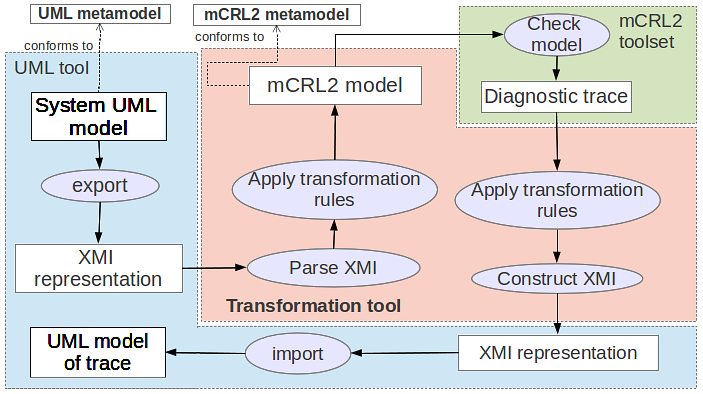
\includegraphics[width=0.7\linewidth,keepaspectratio=true]{./Approach.png}
% \caption{Automated verification of UML models}
% \label{fig:approach}
% \figshrinkend
%\end{figure}

%%The level of sophistication and mathematical background required for using such formalisms is yet another obstacle for adopting formal methods. 
%%In practice, software requirements are written in natural language, and often contain ambiguities, making it difficult even for experienced 
%%practitioners to capture them accurately with temporal logic. There are subtle, but crucial details which are often overlooked and 
%%need to be carefully considered in order to distil the right formula.

% just mention here the patterns, the fact that there are 3 categories of approaches
% tackling the problem, the general deficiencies of these approaches and how we want to
% take the best of all worlds; 
\vspace{-3 pt}
In an attempt to ease the use of temporal logic,
in~\cite{Dwyer:1999:PPS:302405.302672}, a pattern-based classification
was developed for capturing requirements and generating input to model
checking tools. The authors observed that almost
all ($>500$)  properties they surveyed can be mapped into one of several
property patterns. Each pattern is a high-level, formalism-independent
abstraction and captures a commonly occurring requirement. Their
hierarchical taxonomy is based on the idea that each pattern has a
\emph{scope}, which defines the extent of program execution over which
the pattern must hold, and a \emph{behavior}, which describes the
intent of the pattern. The pattern system identifies 5 scopes and 11
behavior variations that can be combined to create 55 different property
templates. Examples of scopes are: \emph{globally}, and \emph{after}
an event or state occurs; examples of behavior classification are:
\emph{absence} (an event or state should never occur during an execution)
and \emph{response} (an event or state must be followed by another event
or state).

\vspace{-3 pt}
Although the patterns website~\cite{PSP} contains a collection
of mappings for different target formalisms such as LTL and CTL, 
in practice practitioners have to fully understand the
solutions before they can select and apply the appropriate ones.
%%Based on investigating over 500 properties coming from different domains,
%%and specified in several formalisms, a pattern-based classification was
%%developed in~\cite{Dwyer:1999:PPS:302405.302672}. The authors observed
%%that almost all the surveyed properties can be mapped into one of several
%%property patterns. Each pattern is a high-level, formalism-independent
%%abstraction that captures a commonly occurring requirement. These patterns
%%can be instantiated with specific events or states and then mapped to
%%several different formalisms for model checking tools. Their hierarchical
%%taxonomy is based on the idea that each pattern has a \emph{scope}, which
%%defines the extent of program execution over which the pattern must hold,
%%and a \emph{behavior}, which describes the intent of the pattern. The
%%pattern system identifies 5 scopes and 11 behavior variations that can be
%%combined to create 55 different property templates. Examples of scopes
%%are: globally, before an event or state occurs, after an event or state
%%occurs.  Examples of behavior classification are: absence (an event or
%%state should never occur during an execution), precedence (an event or
%%state always occurs before another one), or response (the occurrence of a
%%an event or state must be followed by another event or state), capturing a
%%cause-effect relation.  Although the patterns website~\cite{PSP} contains
%%a collection of mappings for different target formalisms, such as LTL,
%%CTL, QRE and Graphical Interval Logic, which can be considered helpful,
%%practitioners have to fully understand the provided solutions before
%%they can select and apply the appropriate ones in practice.\medskip
%%
To mitigate this problem, 
several conversational tools~\cite{Smith02propel:an,konrad2005facilitating,Mondragon_prospec}
have been proposed for elucidating properties,
based on the patterns. These tools guide users in
selecting the appropriate pattern and optionally produce
a formula in some target temporal logic.  
%Another category of
%approaches~\cite{Ziemann02anextension,Flake03formalsemantics,Ackermann:2006:LOS:2135315.2135339}
%deal with temporal extensions of the Object Constraint Language
%(OCL), as means to specify system properties. OCL is a declarative
%textual language for describing invariants for classes and
%pre- and postconditions of operations. Although it forms an
%integral part of UML, it lacks the means to specify constraints
%over the dynamic behavior of a model. 
Alternative
approaches~\cite{Autili:2007:GSS:1290845.1290859,Lee97agraphical,Smith:2001:ECG:882477.883639,Knapp:2006:MCU:1762828.1762836,Lilius99vuml:a,Kugler:2005:TLS:2140653.2140692,MVPSA}
tackle the property specification problem by proposing new graphical
notations for specifying properties. 
% A downside of all these approaches is
% that they still expect users to have some expertise in temporal logic.
As far as we have been able to trace, all approaches deal with state-based logics. Such
logics conceptually do not match the typical event-based UML sequence
diagrams and activity diagrams, in which events represent methods calls
or asynchronous communication between distributed components.

The contribution of our work is a simplification of the process of specifying
functional requirements for event-based systems.  We introduce PASS,
a Property ASSistant which is a tool that guides and facilitates 
deriving system properties. Our starting point was the pattern
system~\cite{Dwyer:1999:PPS:302405.302672}, which we extended with over
50 useful property templates. 
The pattern templates instantiated with PASS have three notations:
a natural language summary, a $\mu$-calculus formula and a UML sequence
diagram depicting desired behaviors.  We utilized mCRL2's rich data
extensions of the $\mu$-calculus to express complex data-dependent
properties.  Lastly, we automatically generate
monitors which can be used for property-driven on-the-fly state space 
exploration using the standard exploration facilities of mCRL2.
Our monitors are essentially sequence diagrams, acting as
observers of message exchanges.

\vspace{-3 pt}
We deliberately chose to develop PASS as an Eclipse plug-in, as
our strong motivation was to stay within an existing UML development
environment, rather than use an external helper tool for this.  We are
convinced that this increases the tool accessibility by allowing software
engineers to remain focused in the realm of UML designs.  In addition,
a tight connection between elements of the design and instances of the property
template is kept, such that, if the design is changed, these changes can
be easily propagated in the property template placeholders.  To this end,
we use the standard MDT-UML2~\cite{MDTUML2} Eclipse modeling API.
%Our strong
%motivation was to stay in the same UML development environment, rather
%than use an external helper tool for this.  It should increase the tool
%accessibility by allowing software engineers to remain focused in the
%realm of UML designs.  In addition, a tight bond between elements of
%the design and instances of the property template is kept, such that,
%if the design is changed, these changes can be easily propagated in
%the property template placeholders.  To this end, we use the standard
%MDT-UML2~\cite{MDTUML2} Eclipse modeling API. Our tool is developed
%as an Eclipse plugin.  Second, the pattern templates instantiated with
%PASS have three notations: a natural language summary, a $\mu$-calculus
%formula and a UML sequence diagram depicting the desired behavior. Most
%approaches to date have focused on LTL, which is a state-based temporal
%logic formalism. Conversely, the $\mu$-calculus is event-based, and as
%such is a good match for the sequence diagrams notation.  These events can
%represent methods calls or asynchronous communication between distributed
%components.  Moreover, such communication is data-dependent, which is why
%we introduce the possibility to define quantifiers, to express complex
%properties in a concise manner, e.g., every element of a certain type
%must fulfil a certain property.  Unlike LTL or CTL,  the $\mu$-calculus
%is powerful enough to achieve this in a natural way. Third, to cope with
%state-space explosion, we provide one additional automatically-generated
%notation: a monitor for on-the-fly model checking, or bug hunting.
%We interpret a sequence diagram as an observer of the message exchanges
%in the system.  This helps to avoid exploring irrelevant parts of
%the state space. The state space generation is thus property driven,
%and stops as soon as an error is found.  
We revisit a case study we did previously
in~\cite{DBLP:dblp_conf/nfm/RemenskaTWHVCB13}, this time using PASS
to obtain the formula and monitor for checking the
property.\medskip
\vspace{-3 pt}

\noindent\emph{Structure.}
In Section~\ref{sec:RelatedWork} we
% survey the most relevant related approaches,
survey related approaches,
and outline their advantages and
% shortcomings. Section~\ref{sec:Preliminaries} briefly introduces
shortcomings. Section~\ref{sec:Preliminaries} introduces
mCRL2, $\mu$-calculus and UML sequence
diagrams. We describe our approach in Section~\ref{sec:Approach}.
In Section~\ref{sec:CaseStudy} we apply PASS on a case study from the
Grid domain, and we conclude in Section~\ref{sec:Conclusions}.
\vspace{-7 pt}

\section{Related Work}
\vspace{-7 pt}

\label{sec:RelatedWork}
PROPEL~\cite{Smith02propel:an} is a tool that
guides users in selecting the appropriate template from the patterns
classification. PROPEL adds new patterns covering subtle aspects
not addressed by the patterns classification of~\cite{Dwyer:1999:PPS:302405.302672} (such as considering the effect
of multiple occurrences of a cause in a pattern); at the same time it
omits patterns such as the universality, bounded
existence and chain patterns. The resulting templates are represented
using ``disciplined natural language'' and finite state automata rather
than temporal logic expressions.
%
%Recognizing that there are subtle aspects not covered
%by the original patterns, such as what happens in a response property
%if the cause occurs multiple times before the effect takes place, they
%extended them with variants. The resulting templates are represented
%using ``disciplined natural language'' and finite state automata.
%PROPEL does not support the universality, bounded existence, and
%the chain patterns, nor does it generate formulas in any of
%the commonly used temporal logic formalisms.  
Similar to PROPEL, the tools SPIDER~\cite{konrad2005facilitating}
and Prospec~\cite{Mondragon_prospec} extend the original patterns but
add compositionality.  SPIDER is no longer maintained and
available; the latest version of Prospec that we found and tested
(Fig.~\ref{fig:Approaches} left) produces formulas in Future Interval
Logic, not LTL as stated in~\cite{Mondragon_prospec}.

Approaches that use a graphical notation for specifying properties
come closest to the realm of modeling the system behavior.
In~\cite{Lee97agraphical}, formulas are represented as acyclic graphs of
states and temporal operators as nodes.  Technically, the underlying LTL
formalism is hidden from the user but the notation still closely resembles
the formalism.  As such, it is not very accessible.  Another tool,
called the TimeLine Editor~\cite{Smith:2001:ECG:882477.883639} permits
formalizing specific requirements using timeline diagrams. For instance,
response formulas are depicted in timeline diagrams by specifying
temporal relations among events and constraints.  These diagrams are
then automatically converted into B\"uchi automata, amenable to model
checking with SPIN.  Unfortunately the tool is no longer available.
\begin{figure*}[h!]
  \centering
  \subfloat{\label{fig:Prospec}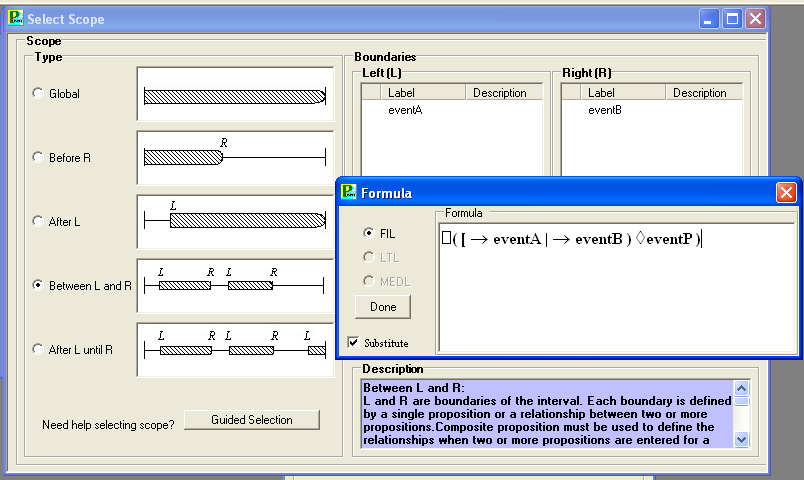
\includegraphics[width=0.73\linewidth]{./Prospec.png}}    
  \hfill
  \subfloat{\label{fig:Charmy}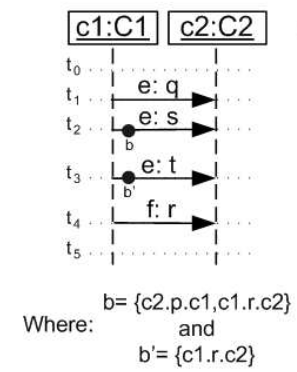
\includegraphics[width =0.26\linewidth]{./Charmy.png}}
  \caption{Left: Prospec tool; right: CHARMY PSC graphical notation}
  \label{fig:Approaches}
\end{figure*}
The CHARMY approach~\cite{Autili:2007:GSS:1290845.1290859} presents
a scenario-based visual language called Property Sequence Charts
(PSC). Properties in this language are relations on a set of exchanged
system messages. The language borrows concepts from UML 2.0 Sequence
Diagrams and the tool uses the toolset SPIN as a backend for model checking
generated B\"uchi automata~\cite{Giannakopoulou:2001:AVT:872023.872506}.
The PSC notation uses textual restrictions for past and future events,
placed as circles directly on message arrows (Fig.~\ref{fig:Approaches}
right). A drawback of PSC is that it does not support asynchronous
communication, which is omnipresent in concurrent systems.  Furthermore,
CHARMY is a standalone framework for architectural descriptions, not
inter-operable with UML tools. As such, its use in industrial contexts
is limited.

Among the UML-based tools are
HUGO/RT~\cite{Knapp:2006:MCU:1762828.1762836} and
vUML~\cite{Lilius99vuml:a}.  HUGO/RT is a tool for model checking
UML 2.0 interactions against a model composed of message-exchanging
state machines. The interactions represent the desired properties,
and are translated together with the system model into B\"uchi automata
% for model checking with SPIN.  The version we tested neither supports
for model checking with SPIN.  The version we tested supports no
asynchronous messages nor combined fragments.  vUML~\cite{Lilius99vuml:a}
is, like HUGO/RT, essentially a tool for automating verifications
of UML state machines.  Properties must be specified in terms of
% undesired scenarios.  The verification is based on checking whether
% it is possible to reach error states. This is inconvenient, as users
undesired scenarios.  The verification is based on the ability
to reach error states. This is inconvenient, as users
must specify these manually.  Live Sequence Charts (LSC) are also
used~\cite{Kugler:2005:TLS:2140653.2140692,MVPSA} as a graphical
formalism for expressing behavioral properties.  They can distinguish
between possible (cold) and mandatory (hot) behaviors.  For both, B\"uchi
automata and LTL formulas are generated automatically from the diagrams.
UML 2.0 sequence diagrams borrow many concepts from LSC, by introducing
% the \emph{assert} and \emph{negate} fragments to capture mandatory and
% forbidden behavior. On the other hand, LSCs lack many UML features.
the \emph{assert} and \emph{negate} fragments capturing mandatory and
forbidden behavior. However, LSCs lack many UML features.
  
  Finally, there are several temporal extensions of UML's property
  language OCL. Resembling an OO programming language, OCL constraints
quickly become quite dense and cryptic, and editing them manually is
error-prone. Another problem is the extent to which designers are
familiar with this language.  Finally, OCL is by itself incapable
of reasoning about temporal behavior.  In~\cite{Ziemann02anextension}
temporal modifiers @pre and @next are introduced for specifying past and
future state-oriented constraints.  
% In~\cite{Flake03formalsemantics},
% a real-time constraint extension of OCL is proposed for models described
% by UML state machines; they claim to be able to describe all the existing
% patterns in these OCL expressions. 
To simplify constraint definitions
with OCL, \cite{Ackermann:2006:LOS:2135315.2135339} proposes 
to use specification patterns for which OCL constraints can be generated
automatically.  The behavioral specification of software components refers
to interface specifications, which are not really dynamic views. Moreover,
this work does not introduce means to specify temporal properties.
\vspace{-7 pt}

\section{Preliminaries}
\label{sec:Preliminaries}
%\subsection{Property Patterns}
\vspace{-7 pt}

\subsection{Brief Introduction to mCRL2 and $\mu$-calculus}
mCRL2 is a language and accompanying toolset for specifying and analyzing concurrent systems. 
Our choice for using the mCRL2 language is motivated by its rich set of 
abstract data types as first-class citizens, as well as its powerful toolset for analyzing, simulating, and visualizing specifications. 
The fragment of the mCRL2 syntax that is most commonly used is given by the following BNF grammar:
\vspace{-7 pt}
% \[p ::= a(d_1,\dots,d_n) \mid \tau \mid \delta \mid p+p \mid p\cdot p \mid p||p \mid \sum\nolimits_{d:D}p \mid c\rightarrow p\diamond p \mid \nabla_H(p) \mid \Gamma_C(p)
% \]
\[p ::= a(d_1,\dots,d_n) \mid \tau \mid \delta \mid p+p \mid p\cdot p \mid p||p \mid \sum\nolimits_{d:D}p \mid c\rightarrow p\diamond p
\]
Actions are the basic ingredients for models. They represent some observable
atomic event. An action $a$ of a process may have a number of data arguments  \begin{math}d_1,...,d_n\end{math}.
The action ${\tau}$ denotes an internal step, which cannot be observed from the external world. 
Non-deterministic choice between two processes
is denoted by the ``$+$'' operator. Processes can be composed sequentially and in parallel by means of ``$\cdot$'' and
``${||}$''. The sum
operator $\sum_{d:D}p$ denotes choice among
processes parameterized by variable $d$. The behavior of the conditional process $c\rightarrow p\diamond p$ 
depends on the value of the boolean expression $c$: if it evaluates to true, process $p$
is chosen and otherwise process $q$ is chosen.
This allows for modeling systems whose behavior is data-dependent.
% To enforce synchronization between processes, the allow operator ${\nabla_H(p)}$ specifies the set of actions $H$ that are allowed
% to occur. To show possible communications in a system and the resulting actions, the communication operator
% ${\Gamma_C(p)}$ is used. The elements of set $C$ are so-called multi-actions of the form $a_1\ |\ a_2\ |\ \dots |\ a_n \rightarrow c$, which intuitively
% means that action $c$ is the result of the multi-party synchronization of actions $a_1 , a_2 , \dots $ and $a_n$.
There are a number of built-in data types in mCRL2, such as integers,
reals, booleans, lists, and sets. 
Furthermore, by a \textbf{sort} definition one can define a new data type. Recursive process 
equations can be declared by \textbf{proc}.

The semantics associated with the mCRL2 syntax is a Labeled Transition System (LTS)
that has multi-action labeled transitions, which can carry data parameters. The language used by the mCRL2
toolset for model checking specific properties is an extension of the modal
$\mu$-calculus~\cite{Emerson97modelchecking}. This formalism stands out from most modal and temporal logic formalisms with respect to its
expressive power. Temporal logics like LTL, CTL and CTL* all have translations~\cite{cranen2011linear} into $\mu$-calculus,
witnessing its generality. This expressiveness comes at a cost: very complex formulas with no intuitive and apparent interpretation can be coined. 
The syntax of mCRL2's modal $\mu$-calculus formulas we are concerned with in this paper
is defined by the following grammar:
\vspace{-5 pt}
\[
\begin{array}{ll}
\phi & ::= b \mid \phi\wedge\phi \mid \phi\vee\phi \mid \forall d{:}D.~\phi \mid \exists d{:}D.~\phi
\mid [\rho]\phi \mid \langle\rho\rangle\phi \mid \mu Z\ldotp\phi(Z) \mid \nu Z\ldotp\phi(Z) \\
\rho & ::= \alpha \mid nil \mid \rho\cdot\rho \mid \rho^* \mid \rho^+ \\
\alpha & ::= a(d_1,\dots,d_n) \mid b \mid \neg \alpha \mid \alpha\cap\alpha \mid 
\alpha\cup\alpha \mid \bigcap{d{:}D}.~\alpha \mid \bigcup{d{:}D}.~\alpha \\
\end{array}
\]
Properties are expressed by state formulas $\phi$, which contain
Boolean data terms $b$ that evaluate to true or false and which can contain data variables, the
standard logical connectives \emph{and} ($\land$) and \emph{or}
($\lor$), the modal operators \emph{must} ($[\_]\_$) and \emph{may}
($\langle \_\rangle\_$), and the least and greatest fixpoint operators
$\mu$ and $\nu$. In addition to these, mCRL2's extensions add universal
and existential quantifiers $\forall$ and $\exists$.

The modal operators take regular expressions
$\rho$ for describing words of actions, built up from the empty word $nil$, individual
actions described by an action formula $\alpha$, word
concatenation $\rho \cdot \rho$ and (arbitrary) iteration of words $\rho^*$ and $\rho^+$.
Action formulas describe sets of actions; these sets are built up from the empty
set of actions (in case Boolean expression $b$ evaluates to false), the set of all possible actions
(in case Boolean expression $b$ evaluates to true); individual actions $a(d_1,\dots,d_n)$, 
action complementation and finite and possibly infinite intersection $\cap$ and union $\cup$.
A state of an LTS (described by an mCRL2 process) satisfies $\langle \rho \rangle \phi$
iff from that state, there is at least one transition sequence matching $\rho$,
leading to a state satisfying $\phi$;
$[\rho]\phi$ is satisfied by a state iff all transition sequences matching $\rho$ starting in that 
state lead to states satisfying $\phi$.
For instance, $[\neg (\bigcup{n{:}Nat}.~
\textit{read}(n+n))]\textit{false}$ states that a process should not execute any actions
other than read actions with even-valued natural numbers.
Note that $[a]\phi$ is trivially satisfied in states with no ``\emph{a}''-transitions.

In mCRL2, verification of $\mu$-calculus formulas is conducted using tooling that operates
on systems of fixpoint equations over first-order logic expressions.
This sometimes requires too much overhead to serve as a basis for lightweight 
bug-hunting, as it can be difficult to interpret the counterexamples that are obtained from
these equation systems in terms of the original mCRL2 process.
Observers, or monitors (\`{a} la B\"uchi) defined in the mCRL2 model itself, can sometimes
be used to bypass the problem.
However, not all $\mu$-calculus formulas are amenable to such a conversion.
\vspace{-10 pt}

\subsection{UML Sequence Diagrams}
\vspace{-6 pt}

Sequence diagrams model the interaction among a set of components, with
emphasis on the sequence of \emph{messages} exchanged over time. Graphically, they have
two dimensions: the objects participating in the scenarios are placed horizontally, 
while time flows in the vertical dimension. The participants are shown as rectangular boxes, with the vertical lines
emanating from them known as \emph{lifelines}. 
Each message sent between the lifelines defines a specific communication, synchronous or asynchronous.
Messages are shown as horizontal arrows from the lifeline of the sender to the lifeline of the receiver instance. 

Sequence diagrams have been considerably extended in UML 2.x to allow expressing of complex control 
flows such as branching, iterations, and referring to existing interactions.
\textbf{Combined fragments} are used for this purpose. The specification
supports different fragment types, with operators such as \emph{alt, opt, loop, break, par}. They are
visualized as rectangles with a keyword indicating the type.
Each combined fragment consists of one or more interaction operands. Depending
on the type of the fragment, constraints can guard each of the interaction operands. 
Combined fragments can be nested with an arbitrary nesting
depth, to capture complex workflows. Figure~\ref{fig:SDExample} shows how some of them can be
used. 
\begin{figure}[!t]
\centering
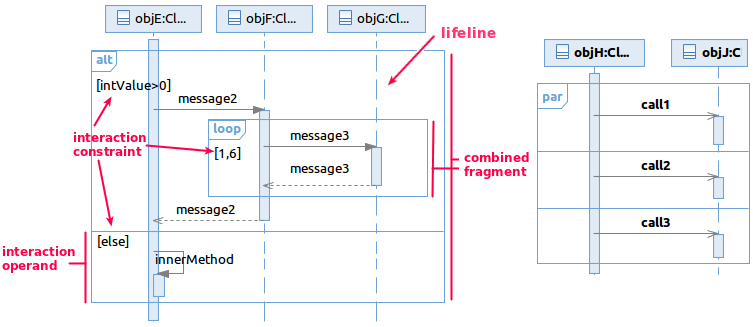
\includegraphics[width=1.0\linewidth,keepaspectratio=true]{./Figure2_merged.png}
\caption{Sequence diagrams with combined fragments}
\label{fig:SDExample}
\end{figure}

There are also two less-known combined fragments: \emph{assert} and \emph{neg}. Their use in practice
is limited, because their semantics described in the UML 2.0 superstructure specification~\cite{UML2.4_superstructure}
are rather vague and confusing. By default, sequence diagrams without the use of these two operators 
only reflect possible behavior, while \emph{assert} and \emph{neg} alter the way 
a trace can be classified as valid or invalid. The specification characterizes
the semantics of a sequence diagram as a pair of valid and invalid traces,
where a trace is a sequence of events or messages.
The potential problems with the UML 2.0 assertion and negation are explained in~\cite{Harel07assertand}.
In summary, the specification aims at depicting of required and forbidden behaviors.
However, as~\cite{Harel07assertand} points out, stating that ``the sequences of the operand of the assertion are the only valid continuations. All other continuations result in an invalid trace''
suggests that the invalid set of traces for an \emph{assert} fragment is its complement, i.e., the set of all other possible traces.
Conversely, the standard also declares that the
invalid set of traces are associated only with the use of
a \emph{neg} fragment, which is contradictory.
For this reason, we also believe that these two operators should rather be considered 
as modalities. We restrict their usage to single events in property specifications, and assign the following semantics:
\emph{neg} is considered a set-complement operator for the event captured by the fragment, while \emph{assert}
specifies that an event must occur. In addition, we
disallow nestings between these two fragments.
We find that this does not limit the expressiveness of property specifications in practice.
\vspace{-6 pt}
\section{The Approach}
\label{sec:Approach}
\vspace{-7 pt}

\subsection{The Rationale}
\vspace{-5 pt}
To describe our proposal to a correct and straightforward property elucidation,
we outline the motivations behind the choices we made, and how they differ from
existing related approaches. 
%
% TW: removed because of repetition...
%As already stated, to bridge the gap between everyday practical software 
%requirements specification and the property patterns classification,
%several conversational tools have already been proposed. 

While we follow 
on the idea of using a guiding questionnaire to incrementally refine various aspects
of a requirement, we find the resulting artifacts (LTL formulas or graphical representations of finite state machines) from using the available ones 
(discussed in Section~\ref{sec:RelatedWork}) not yet suitable for practical application in our context.
For one, the practitioner must manually define the events to be associated with the placeholders when 
instantiating the template. To avoid potential errors, as well as
reduce effort in specifications, we want to ideally stay in the same IDE used
for modeling the system, and select only existing events that represent
valid communication between components.  
In addition, we can already obtain mCRL2 models from UML designs comprising sequence diagrams~\cite{DBLP:dblp_conf/nfm/RemenskaTWHVCB13}.
In our experience, visual scenarios are the most suitable and commonly used  
means to specify the dynamics of a system. 
We believe that such a visual depiction of a scenario, more than finite state machines, 
improves the practitioner's understanding of the requirement as well. 
This is why we chose sequence diagrams as a property specification artifact too.

Most of the invented notations used by existing scenario approaches can fit well in UML 2.0 sequence diagrams.
Profiles are a standard way to extend UML for expressing concepts not included in the official metamodel. 
In short, UML profiles consist of stereotypes that can be applied to any UML model, like classes,
associations, or messages. We used this mechanism 
to apply the restrictions on the usage of \emph{neg} and \emph{assert},
as well as to distinguish between events presenting interval bounds and regular ones, from the patterns.
As an example, Fig.~\ref{fig:ResponsePattern} depicts the \emph{precedence chain} pattern (with
a \emph{between-Q-and-R} scope), with the stereotypes applied to messages
\emph{Q} and \emph{R}.
The pattern expresses that event \emph{P} must precede the chain of events
\emph{S, T}, always when the system execution is in the scope between events
\emph{Q} and \emph{R}.
We find this a much more intuitive scenario representation than the CHARMY/PSC
one (Fig.~\ref{fig:ResponsePatternCharmy}), for the same pattern.
Notice that we do not have to specify constraints on past unwanted events, as they are automatically
reflected in the $\mu$-calculus formula, as long as there is a distinction between interval-marking messages,
regular, mandatory, and forbidden ones. Also, the CHARMY/PSC notation presents the scenario in a negative form, using ``f:'' to
explicitly mark an error message. 
\begin{figure*}[t!]
  \centering
  \subfloat[Sequence Diagram with monitor]{\label{fig:ResponsePattern}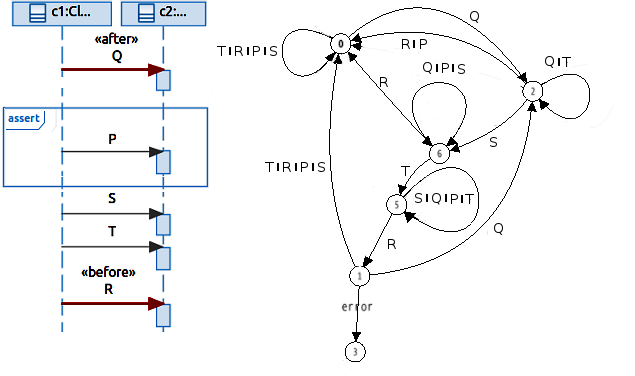
\includegraphics[width=0.62\linewidth]{./ResponseChain_withMonitor1.png}}    
  \hfill
  \subfloat[PSC with B\"uchi automaton~\cite{Autili:2007:GSS:1290845.1290859}]{\label{fig:ResponsePatternCharmy}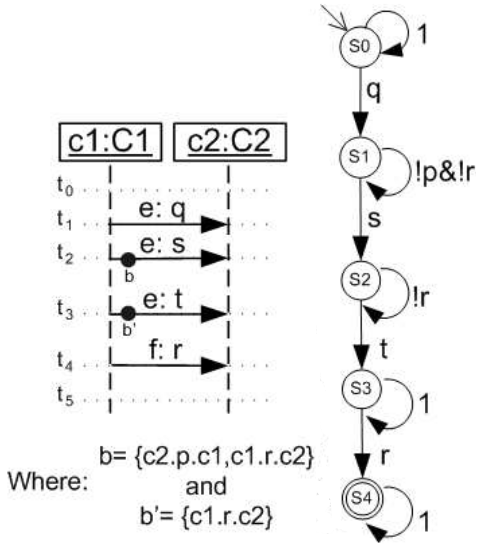
\includegraphics[width =0.38\linewidth]{./ResponseChainPSC.png}}
  \caption{Scenarios for the precedence chain pattern}
\end{figure*}

Furthermore, most visual scenario approaches cover the (state-based) LTL mappings and extensions of the pattern system. 
Event-based temporal logics have not received much attention. Even though the original pattern 
system does not cover $\mu$-calculus, such mappings~\cite{RAFMC} have been developed by the CADP team.
% However, there are no pattern extensions available.
These are adequate for action- or event-based systems,
making them a good match for sequence diagrams, where communication between components is depicted.
LTL logic is interpreted over Kripke structures, where the states are labeled with elementary 
propositions that hold in each state, while $\mu$-calculus is interpreted over LTS-es, in which the transitions
are labeled with actions that represent state changes.
Even though both are complementary representations of the more general finite state automata, 
conversions between them are not practical, as they usually lead to a significant state space increase. 
For example, the fact that a lock has
been acquired or released can be naturally expressed by actions. Since state-based
temporal logics lack this mechanism, an alternative is to introduce a variable to indicate
the status of the lock, i.e., expose the state information. With such properties, LTS
representations are more intuitive, and easier to query using event-based logics.
\vspace{-1 pt}

Given that communication among components proceeds via actions (or events) which can
represent synchronous or asynchronous communication, property specification
can be defined over sequences of actions that are data-dependent.
Fortunately, $\mu$-calculus is rich enough to express both state and action formulas,
and provides means for quantification over data, which many formalisms lack. 
%maybe this can go to the questionnaire?
For example, with our approach, a practitioner can use 
a wild-card ``*'' to express that the property should be evaluated for all values
that message parameters can carry. This allows us to use patterns which would otherwise
make sense only for state-based formalisms. For example, the \emph{universality}
pattern is used to describe a portion of the system's execution which contains only states/events that have a desired property.
Checking if a certain event is executed in every step of the system execution is not useful most of the time,
so we adapted it in the context of $\mu$-calculus. 
\vspace{-1 pt}

Finally, for the purpose of on-the-fly verification, we provide an
automatically generated mCRL2 monitor which corresponds to the property formula.
We interpret a sequence diagram as an observer of
the message exchanges in the system. This helps in avoiding generation of those
parts of the state space for which it is certain that they do not compose with the
property monitor. In addition, although mCRL2 offers direct model checking
with $\mu$-calculus and can provide feedback when the property fails to hold, this
feedback is not at the level of the mCRL2 process specification.
Using the monitor, the counter-example will be provided at the UML level.

Although any mature visual UML modeling tool 
can be used, we chose IBM's Rational Software Architect (RSA) environment.
One of the advantages is that RSA is built on top of Eclipse, making 
it relatively easy to extend the functionality. To this end, PASS is developed as an Eclipse plug-in, using the 
lightweight UML profile, and as such is available (Fig.~\ref{fig:PASSlaunch}) to any Eclipse-based UML tool.

\vspace{-10 pt}
\subsection{Transforming a $\mu$-calculus Formula Into a Monitor Process} 
\vspace{-5 pt}
A general model checking mechanism used with tools like SPIN 
is to construct a B\"uchi automaton for an LTL formula, which accepts exactly those executions
that violate the property. A product of the model state space (typically a Kripke structure) and the B\"uchi automaton is then composed, 
and checked for emptiness. 
Although syntactically B\"uchi is similar to the finite-state monitor for which we aim,
the difference lies in the acceptance conditions: a monitor accepts only 
finite runs of the system, while B\"uchi can trap infinite executions through
detection of cycles, but potentially needs the entire state space
generated in the process. Runtime verification
does not store the entire state space of a model, so it cannot detect such cycles. 
In addition, to expose state information, transitions in Fig.~\ref{fig:Buchi} are labeled with elementary
propositions rather than actions (notice the $\wedge$ operator). 
As such, we cannot use existing tools for constructing B\"uchi automata with our
approach.
\begin{figure}[!t]
 \centering
\begin{minipage}[!t]{0.5\linewidth}
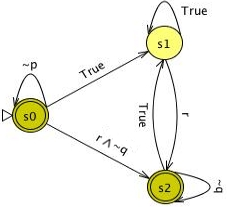
\includegraphics[width=0.6\textwidth]{./Buchi2.jpg}%
\caption{A B\"uchi automaton}
\label{fig:Buchi}
\end{minipage}%
\begin{minipage}[!t]{0.5\linewidth}
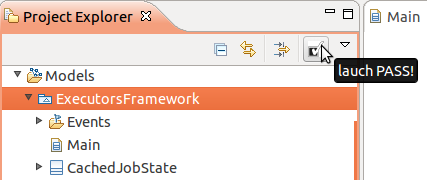
\includegraphics[width=1.0\textwidth]{./PASSlaunch.png}%
\label{fig:PASSlaunch}
\captionof{figure}{Launching PASS from the Eclipse Project Explorer\label{fig:PASSlaunch}}%
% \caption{Launching PASS from the Eclipse Project Explorer}
\end{minipage}
\end{figure}

Not every property can be monitored at runtime when only a finite run has been 
observed so far. Monitorable properties are those for which a violation occurs along a finite execution.
This problem has been studied~\cite{DBLP:journals/corr/abs-1006-3638}, and it is known that the class of 
monitorable properties is strictly larger than
% the commonly believed class
that of \emph{safety} properties.
However, an exact categorization of monitorable properties is missing.
In particular, the definition of \emph{liveness} requires that any finite system
execution must be extendable to an infinite one that satisfies the property. 
By defining an end-scope of a property, we can also assert
violations to \emph{existence} patterns, which are typically in the \emph{liveness} category. 
Such runtime monitor can also assert \emph{universality} and \emph{absence} patterns 
with or without scope combinations. We found that we are able to construct 
a monitor for about 50\% of the property patterns.

We translate a core fragment of the $\mu$-calculus to mCRL2 processes which
can subsequently serve as an observer processes for monitorable properties.
The idea behind the translation is that a violation of a property of the 
form $[\alpha]\phi$ is witnessed by an action that matches the action
formula $\alpha$.  A monitor for such a formula synchronizes
with precisely those actions matching $\alpha$. This generalizes
to sequences of actions matching words described by some $\rho$ for
formulas of the form $[\rho]\phi$.
We restrict to the following grammar:
\vspace{-4 pt}
\[
\begin{array}{ll}
\phi & ::= b \mid \forall d{:}D.\phi \mid [\rho]\phi \mid \phi\wedge \phi\\
\rho & ::= \alpha \mid nil \mid \rho\cdot \rho \mid
              \rho+\rho \mid
              \rho^* \mid \rho^+ \\
\alpha & ::=  a(d_1,\dots,d_n) \mid \neg \alpha \mid b \mid
              \alpha \cap \alpha \mid \alpha \cup \alpha \mid
              \bigcap d{:}D.~\alpha \mid \bigcup d{:}D.~\alpha
\end{array}
\]
Before we present the translation, we convert the formulas in
guarded form. That is, we remove every occurrence of $\rho^*$ and $nil$ using
the following rules:
\[
\vspace{-4 pt}
\begin{array}{lclr}
[nil]\phi = \phi & \qquad\qquad
[\rho^*]\phi = [nil]\phi \wedge [\rho^+]\phi & \qquad\qquad\qquad\qquad\qquad\qquad\qquad (1)
\end{array}
\]
The function $\Tr$ takes two arguments (a formula and a list of typed
variables) and produces a process. It is defined inductively as follows:
\[
\begin{array}{lll}
\Tr_l(b) &= (\neg b \to \textit{error}) & \qquad\qquad\qquad\qquad\qquad\qquad\qquad (2)\\ 
\Tr_l(\forall d:D.\phi_1) & = \sum d{:}D. \Tr_{l\concat [d:D]} (\phi_1) & \qquad\qquad\qquad\qquad\qquad\qquad\qquad (3)\\
\Tr_l(\phi_1 \wedge \phi_2) & = \Tr_l(\phi_1) + \Tr_l(\phi_2) & \qquad\qquad\qquad\qquad\qquad\qquad\qquad (4)\\
\Tr_l([\rho]\phi_1) & = \TrR_l(\rho) \cdot \Tr_l(\phi) & \qquad\qquad\qquad\qquad\qquad\qquad\qquad (5)\\
\end{array}
\]
where $\TrR$ takes a regular expression (and a list of typed variables)
and produces a process or a condition:
\[
\begin{array}{llr}
\TrR_l(\alpha) &= \bigoplus\limits_{a \in Act} (\sum d_a{:}D_a.~ \TrA_l(a(d_a),\alpha) \to a(d_a)) & (6)\\
\TrR_l(\rho_1 \cdot \rho_2) & = \TrR_l(\rho_1) \cdot \TrR_l(\rho_2) & (7)\\
\TrR_l(\rho_1 + \rho_2) &= \TrR_l(\rho_1) + \TrR_l(\rho_2) & (8)\\
\TrR_l(\rho^+) & = X(l) \qquad \textit{where $X(l) = \TrR_l(\rho)\cdot X(l)$ is
a recursive process} & (9)
\end{array}
\]
where $\bigoplus$ is a finite summation over all action names
$a \in Act$ of the mCRL2 process and
where $\TrA$ takes an action and an action formula and produces a condition
that describes when the action is among the set of actions described by
the action formula:
\vspace{-5 pt}
\[
\begin{array}{llr}
\TrA_l(a(d_a),a'(e)) & = \left \{ \begin{array}{ll} d_a = e & \text{if a = a'}\\
                                  \text{false} & \text{otherwise}\\
                                  \end{array} \right .& \qquad\qquad (10)\\
\TrA_l(a(d_a),b) & = b & \qquad\qquad (11)\\
\TrA_l(a(d_a),\neg \alpha) & = \neg \TrA_l(a(d_a),\alpha) & \qquad\qquad (12)\\
\TrA_l(a(d_a),\alpha_1 \cap \alpha_2) & =
\TrA_l(a(d_a),\alpha_1) \wedge \TrA_l(a(d_a),\alpha_2) & \qquad\qquad (13)\\
\TrA_l(a(d_a),\alpha_1 \cup \alpha_2) & =
\TrA_l(a(d_a),\alpha_1) \vee \TrA_l(a(d_a),\alpha_2) & \qquad\qquad (14)\\
\TrA_l(a(d_a),\bigcup d{:}D.~\alpha) & = \exists d{:}D.~ \TrA_l(a(d_a),\alpha) & \qquad\qquad (15)\\
\TrA_l(a(d_a),\bigcap d{:}D.~\alpha) & = \forall d{:}D.~ \TrA_l(a(d_a),\alpha) & \qquad\qquad (16)
\end{array}
\]
Using the above translation, Fig.~\ref{fig:ResponsePattern} shows monitor visualization next to the sequence diagram for the precedence chain pattern.
Such a monitor can be placed in parallel with the system model,
to perform runtime verification. Clearly, in the ``worst'' case, if the model is correct with respect to the property,
all relevant model states will be traversed. In practice however, refutation can be found 
quickly after a limited exploration. 
A sketch of such a translation applied on a model with actions \textit{action\_1}, \textit{action\_2},\dots,\textit{action\_n} is shown in Fig.~\ref{fig:MonitorConstruction}.
\begin{figure}[!t]
\centering
{%
\setlength{\fboxsep}{1.5pt}%
\setlength{\fboxrule}{0.5pt}%
\fbox{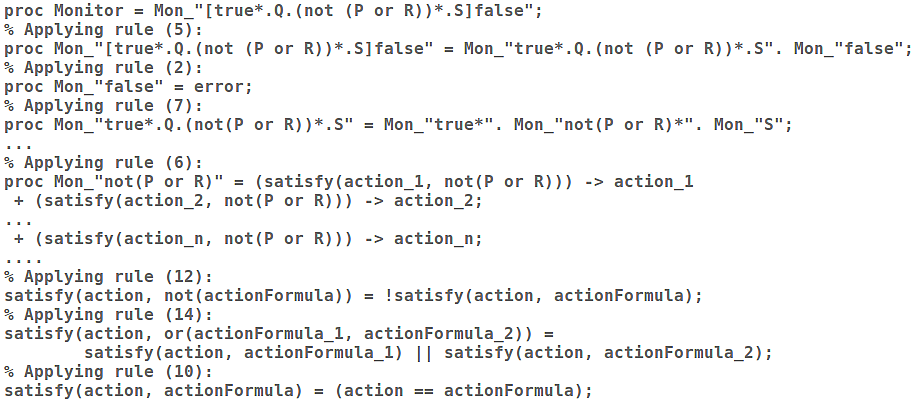
\includegraphics[width=1.0\linewidth,keepaspectratio=true]{./MonitorConstruction.png}}%
}%
\caption{Transforming a $\mu$-calculus formula into a monitor}
\label{fig:MonitorConstruction}
\vspace{-6 pt}
\end{figure}
Intuitively, the monitor process will step through those exact actions that the original system takes. If a sequence of steps refuting the formula is completed,
the monitor will execute the ``error'' action as a last step, indicating that a counter-example trace has been found.
More examples of monitors along with references to
the applied transformation rules in each step, can be found at~\cite{repo:PASS}.
\vspace{-10 pt}
\section{Case Study: DIRAC's Executor Framework revisited}
\vspace{-8 pt}
DIRAC \cite{DIRAC_CommGridSolution} is the grid framework used to support production activities of the LHCb experiment at CERN.
All major LHCb tasks, such as raw data transfer from the experiment's detector to the grid storage, data processing, and user analysis,
are covered by DIRAC. 
Jobs submitted via its interface undergo several processing steps between the moment they are submitted, 
to the point when they execute on the grid. 

The crucial Workload Management components responsible for orchestrating this process are the \emph{ExecutorDispatcher} and 
the \emph{Executors}. Executors process any task sent to them by the ExecutorDispatcher, each one being responsible for a different step in the handling of tasks
(such as resolving the job's input data).
The ExecutorDispatcher takes care of persisting the state of the tasks and distributing them amongst the Executors, based on the
task requirements. It maintains a queue of tasks waiting to be processed, and other internal data structures to keep track
of the distribution of tasks among the Executors.
During testing, developers experienced certain problems: occasionally, tasks submitted in the system would not get dispatched, despite the fact that their responsible Executors
were idle at the moment. The root cause of this problem could not be identified by testing  with different workload scenarios, nor by analysis of the 
generated logs. 
In~\cite{DBLP:dblp_conf/nfm/RemenskaTWHVCB13} we manually formulated this problem as the following safety property:
\begin{lstlisting}[basicstyle=\sffamily\fontsize{7}{8}\selectfont,showspaces=false,showstringspaces=false,showtabs=false,mathescape]
[true$^*$ .
synch_call(1,ExecutorQueues,$\underline{\hspace*{7pt}}$queues,pushTask(JobPath,taskId,false)).true$^*$.
!(synch_call(1,ExecutorQueues,$\underline{\hspace*{7pt}}$queues,popTask([JobPath])))$^*$.
synch_reply(1,ExecutorDispatcher,$\underline{\hspace*{7pt}}$eDispatch,
$\underline{\hspace*{7pt}}$sendTaskToExecutor_return(OK,0))]false 
\end{lstlisting} 
\vspace{-5 pt}
, meaning that a task pushed in the queue must be processed, i.e., removed from the queue before the ExecutorDispatcher
declares that there are no more tasks for processing.
Explicit model checking was not feasible in this case due to the model size (50 concurrent processes),
so we resorted to writing a standard monitoring process set to run in parallel with the original model.
With a depth-first traversal in mCRL2, we effectively discovered a trace~\cite{DBLP:dblp_conf/nfm/RemenskaTWHVCB13} violating the property within minutes, and
used our tool to import and automatically visualize the counter-example as a sequence diagram in RSA.
Since the bug was reported and fixed, we wanted to check if the problem still persists after the fix, this time using PASS to 
elicit the property.
\vspace{-12 pt}
\label{sec:CaseStudy}
\subsection{PASS: The Property ASSistant} 
\vspace{-5 pt}
To cope with the ambiguity of system requirements, PASS 
guides the practitioner via a series of questions to distinguish the types of scope and 
behavior as a relation between multiple events. By answering these questions, 
one is led to consider some subtle aspects of the property, which are typically 
overlooked when manually specifying the requirement in temporal logic.
The last part of the property (i.e. ``before the ExecutorDispatcher
declares that there are no more tasks for processing'') is easily recognized as a scope restriction,
which the user can choose by selecting the appropriate answer from the Scope Question Tree wizard page.
\begin{figure}[!b]
\centering
{%
\setlength{\fboxsep}{1.5pt}%
\setlength{\fboxrule}{0.5pt}%
\fbox{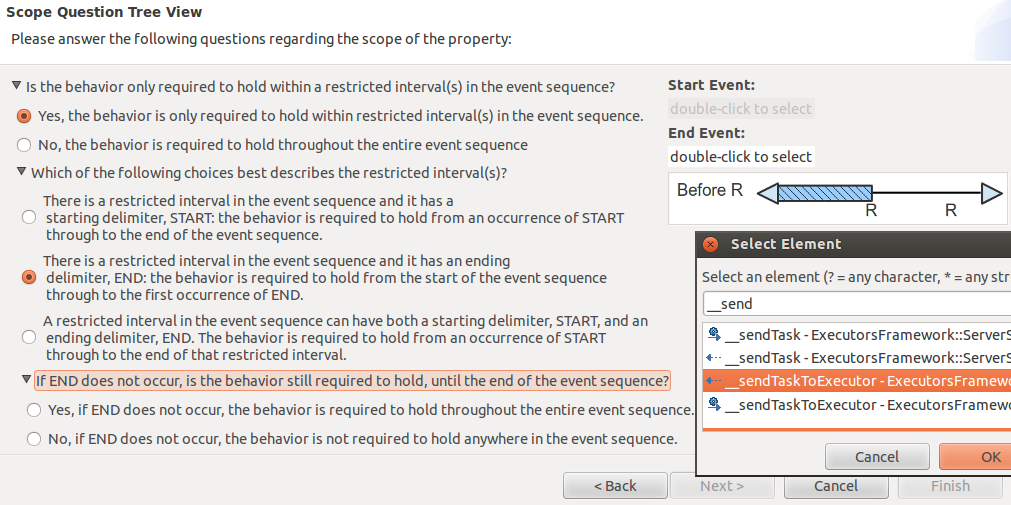
\includegraphics[width=1.0\linewidth,keepaspectratio=true]{./ScopeSelection1.png}}%
}%
\caption{Eliciting the scope for a property with PASS}
\label{fig:ScopePASS}
\end{figure}
This results in a \emph{Before-R} scope restriction, where the actual communication can be selected by double-clicking the end-event placeholder (Fig.~\ref{fig:ScopePASS}).
This presents the user with a popup window with all the possible message exchanges in the model, so he can choose the actual message, in this case
the reply message $\_\_sendTaskToExecutor$.
As already pointed out in~\cite{Smith02propel:an}, a closer examination of the patterns classification reveals some aspects
which are not considered, and may lead to variants in the original scope and behavior definitions. 
For example, the definition of the \emph{Before-R} scope requires that the event \emph{R} necessarily
occurs. This means, if \emph{R} does not occur until the end of the run, the intent or behavior 
of the property could be violated, yet the property as a whole would not be violated 
unless \emph{R} happens. In practice however, it is useful to introduce an \emph{Until-R} variant for cases where the end-delimiter may not occur until the end of 
the system execution. This is captured by the last question in Fig.~\ref{fig:ScopePASS}.
Similar considerations have lead to new variants of the \emph{After-Q-Until-R} and \emph{After-Q-Before-R} patterns.
For instance, whether subsequent occurrences of Q should be ignored, or should effectively reset the beginning of the interval
in which the behavior is considered, are reflected in the questionnaire.
\vspace{-2 pt}

Due to space restrictions we do not show the Behavior Question Tree part of the wizard, although it is easy to
elicit the behavior requirement as a \emph{response} pattern (``a task \emph{pushed} in the queue must be processed, i.e., \emph{removed} from the queue'').
The actual events of interest in this case are \emph{pushTask} and \emph{popTask}. Again, an extension of the pattern system allows
for the user to decide whether the first event (the cause) must necessarily occur in the first place. 
Adding 4 scope and 2 behavior variations have lead to more than 100 ((5+\textbf{4})$\ast$(11+\textbf{2})) unique patterns to be chosen from. 
\vspace{-1 pt}

At the end of the questionnaire, the user is presented (Fig.~\ref{fig:Summary}) with a summary of the requested property, which can be reviewed before making the final decision.
A $\mu$-calculus formula pertaining to the property is presented, along with the possibility to assign concrete parameter values that messages carry. 
Since the property should be evaluated for all possible values of the taskId's domain, a wildcard ``*'' can be used (as shown in the second parameter of \emph{pushTask}).
This assignment results in a formula with a \emph{forall} quantifier. In addition, a sequence diagram (Fig.~\ref{fig:SDProperty}) and a monitor process in mCRL2 (visualized in Fig.~\ref{fig:MonitorProperty} without the data, for clarity)  
are generated, to be used in the final model checking phase.
\begin{figure}[!t]
\centering
{%
\setlength{\fboxsep}{1.5pt}%
\setlength{\fboxrule}{0.5pt}%
\fbox{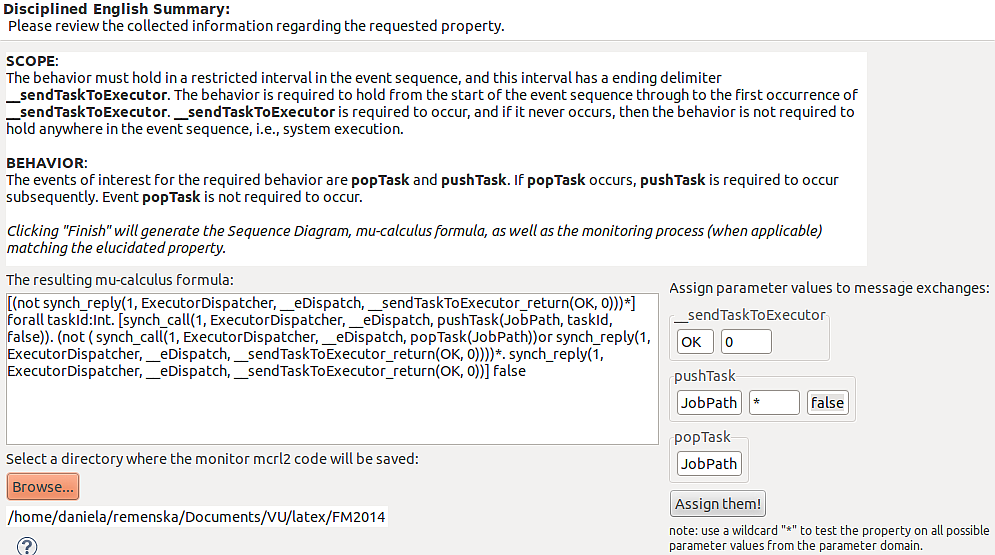
\includegraphics[width=1.0\linewidth,keepaspectratio=true]{./Last.png}}%
}%
\caption{Summary of the elicited property with PASS}
\label{fig:Summary}
\end{figure}
\begin{figure}[!t]
 \centering
\begin{minipage}[!t]{0.5\linewidth}
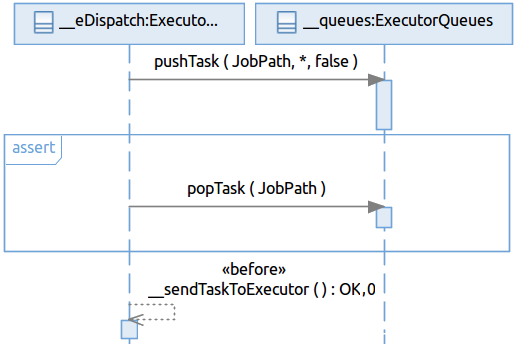
\includegraphics[width=0.95\textwidth]{./SDProperty.png}%
\caption{A sequence diagram for the property}
\label{fig:SDProperty}
\end{minipage}%
\begin{minipage}[t]{0.5\linewidth}
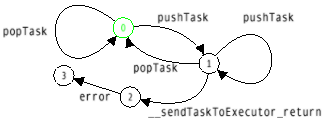
\includegraphics[width=1.0\textwidth]{./PropertyAutomaton.png}%
\captionof{figure}{A monitor for the property\label{fig:MonitorProperty}}%
\end{minipage}
\end{figure}
It is worth noticing that our original manually constructed formula was not entirely correct, and as such could potentially produce spurious counter-examples. 
The general pattern template obtained with PASS is:
\begin{lstlisting}[basicstyle=\sffamily\fontsize{7}{7}\selectfont,showspaces=false,showstringspaces=false,showtabs=false,mathescape]
[(not R)$^*$. P. (not (S or R))$^*$. R] false
\end{lstlisting} 
while the original one was a more restrictive formula of the following form:
\begin{lstlisting}[basicstyle=\sffamily\fontsize{7}{7}\selectfont,showspaces=false,showstringspaces=false,showtabs=false,mathescape]
[true$^*$. P. (not S)$^*$. R] false
\end{lstlisting} 
Using the generated monitor, we performed runtime verification on the corrected model. We linearized the model with the mCRL2 toolset,
and used LTSmin's symbolic reachability tool~\cite{so62465} for efficient state space exploration. LTSmin is language-independent, and can be used as an mCRL2 model checking back-end. 
Taking less than 20 minutes, the symbolic state space explorer 
finished the traversal (2.85 million states) without discovering an \emph{error} step, effectively concluding that the property holds.
The PASS tool, along with the patterns extensions, the model and the monitor of this case study, is available at~\cite{repo:PASS}.
While outside of the current scope, a Java Web Start version of the tool is available for users
who want to elicit a property for existing mCRL2 models created manually and
independently of any UML environment.
% here mention the patterns published, and PASSWebStart?
\vspace{-14 pt}
\section{Conclusions and future work}
\label{sec:Conclusions}
\vspace{-8 pt}
% \lipsum[4-6]
In an effort to automate more aspects of formal verification of distributed
systems, we introduced PASS, a Property ASSistant that brings the process of
correctly specifying 
functional properties closer to software engineers.
Through a series of questions, the practitioner can
consider subtle aspects about a property which are often overlooked.
Motivated by the wish to stay within an existing UML development environment,
rather than use an external helper tool, PASS was developed as an Eclipse plug-in,
thus keeping a strong relationship between the model elements and the property template ones.
Our approach to specifying properties is based on the pattern system~\cite{Dwyer:1999:PPS:302405.302672},
which we extended with useful pattern variations for the event-based $\mu$-calculus
formalism. Besides offering a natural language summary of the elicited property,
a $\mu$-calculus formula and a UML sequence
diagram is provided, depicting the desired behavior. In addition, PASS
automatically generates monitors to be used for efficient property-driven 
runtime verification using the mCRL2 toolset. We believe that automating the property specification process, while keeping
practitioners in their familiar environment, should lead to more active adoption of methods for formal analysis of designs.
We revisited a case study from the grid domain, and discovered that 
despite a reasonably good understanding of $\mu$-calculus, our previously manually
defined property was in fact not fully correct. Using the monitor, we performed runtime verification, which in
the end resorted to full exploration of the state space, and did not disprove the property.

Besides instantiating pattern templates, part of our ongoing work is to define 
a methodology that would allow the experienced practitioner to directly 
write sequence diagrams expressing requirements, based on which a $\mu$-calculus formula and a monitor 
would be provided. 
% Automating performance analysis is on our road-map as well. 
% Profiles are provided as UML extension mechanisms, which allow 
% annotating models with quantitative information (such as expected execution time, resource usage etc.),
% and this mechanism would permit assessing aspects of the system
% such as efficiency and reliability.
% We can use the same target formalism for enhancing the models
% with such quantitative information. The CADP toolset~\cite{DBLP:conf/tacas/GaravelLMS11} for analysis of stochastic
% models is well integrated with mCRL2 for this purpose.
\vspace{-10 pt}
\bibliographystyle{splncs} 
\vspace{-3 pt}
\bibliography{FM2014}
\end{document}


